\documentclass[aspectratio=169]{beamer}
% Add slides directory to search path for Dartmouth theme
\makeatletter
\def\input@path{{../}}
\makeatother
\usetheme{Dartmouth}
\usepackage{graphicx}
\usepackage{tikz}
\usetikzlibrary{shapes.geometric, arrows.meta, positioning, fit, backgrounds}
\usepackage{amsmath}
\usepackage{listings}
\usepackage{xcolor}
\usepackage{booktabs}
\usepackage{hyperref}
\usepackage{tcolorbox}
\usepackage{pgfplots}
\pgfplotsset{compat=1.18}

% Color scheme
\definecolor{darkblue}{RGB}{0,82,155}
\definecolor{lightblue}{RGB}{100,181,246}
\definecolor{darkgreen}{RGB}{46,125,50}
\definecolor{orange}{RGB}{255,152,0}
\definecolor{purple}{RGB}{156,39,176}
\definecolor{teal}{RGB}{0,150,136}

\setbeamercolor{progress bar}{fg=lightblue,bg=lightblue!30}

% Code listing settings
\lstset{
    basicstyle=\ttfamily\scriptsize,
    breaklines=true,
    frame=single,
    backgroundcolor=\color{gray!10},
    keywordstyle=\color{darkblue}\bfseries,
    commentstyle=\color{darkgreen}\itshape,
    stringstyle=\color{orange},
    showstringspaces=false,
    language=Python,
    numbers=left,
    numberstyle=\tiny\color{gray}
}

% Custom boxes
\newtcolorbox{discussionbox}{
    colback=lightblue!10,
    colframe=darkblue,
    title=💬 Discussion Question,
    fonttitle=\bfseries
}

\newtcolorbox{thinkbox}{
    colback=orange!10,
    colframe=orange,
    title=💭 Think About It,
    fonttitle=\bfseries
}

\title{Lecture 22: Mixture of Experts \& Efficiency}
\subtitle{Scaling Efficiently with Sparse Models 🚀}
\author{PSYC 51.07: Models of Language and Communication}
\institute{Dr. Jeremy R. Manning}
\date{Week 9}

\begin{document}

% ============================================================
% TITLE SLIDE
% ============================================================
\begin{frame}[shrink=10]
\titlepage
\end{frame}

% ============================================================
% OVERVIEW
% ============================================================
\begin{frame}[shrink=5]{Today's Journey 🗺️}
\tableofcontents
\end{frame}

% ============================================================
% SECTION 1: THE SCALING PROBLEM
% ============================================================
\section{The Scaling Challenge}

\begin{frame}{The Scaling Dilemma 📈}
\begin{discussionbox}
Larger models perform better... but at what cost?
\end{discussionbox}

\vspace{0.5em}

\textbf{Training a 175B parameter model (GPT-3 scale):}
\begin{itemize}\setlength{\itemsep}{0pt}
    \item 💰 Cost: \$4-12 million in compute
    \item 🔥 Energy: Equivalent to 120 homes for a year
    \item ⏳ Time: Weeks to months on thousands of GPUs
    \item 🐌 Inference: Slow and expensive (\$0.002-0.02 per 1K tokens)
    \item 🌍 Environmental: Massive carbon footprint
\end{itemize}

\vspace{0.5em}

\begin{alertblock}{The Challenge}
Can we get the benefits of scale without the full computational cost?
\end{alertblock}

\vspace{0.3em}

\textbf{Key Insight:} Not all parameters need to be active for every input!
\end{frame}

\begin{frame}[shrink=10]{Dense vs Sparse Models 🎯}
\begin{columns}[T]
\begin{column}{0.48\textwidth}
\textbf{Dense Models (e.g., GPT-3):}

\vspace{0.3em}

\begin{center}
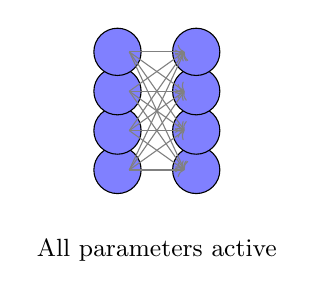
\begin{tikzpicture}[scale=0.5]
    % All neurons active
    \foreach \y in {1,2,3,4} {
        \node[circle, draw, fill=blue!50, minimum size=0.6cm] at (0,\y) {};
        \node[circle, draw, fill=blue!50, minimum size=0.6cm] at (2,\y) {};
    }
    % Connections (all)
    \foreach \i in {1,2,3,4} {
        \foreach \j in {1,2,3,4} {
            \draw[->, gray] (0.3,\i) -- (1.7,\j);
        }
    }
    \node[below] at (1,-0.5) {\small All parameters active};
\end{tikzpicture}
\end{center}

\vspace{0.3em}

\begin{itemize}\setlength{\itemsep}{0pt}
    \item All parameters used
    \item High compute per token
    \item Expensive inference
    \item Simple architecture
\end{itemize}
\end{column}

\begin{column}{0.48\textwidth}
\textbf{Sparse Models (MoE):}

\vspace{0.3em}

\begin{center}
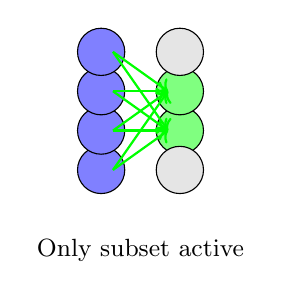
\begin{tikzpicture}[scale=0.5]
    % Only some neurons active
    \foreach \y in {1,2,3,4} {
        \node[circle, draw, fill=blue!50, minimum size=0.6cm] at (0,\y) {};
    }
    \node[circle, draw, fill=green!50, minimum size=0.6cm] at (2,2) {};
    \node[circle, draw, fill=green!50, minimum size=0.6cm] at (2,3) {};
    \node[circle, draw, fill=gray!20, minimum size=0.6cm] at (2,1) {};
    \node[circle, draw, fill=gray!20, minimum size=0.6cm] at (2,4) {};
    % Connections (sparse)
    \foreach \i in {1,2,3,4} {
        \draw[->, green, thick] (0.3,\i) -- (1.7,2);
        \draw[->, green, thick] (0.3,\i) -- (1.7,3);
    }
    \node[below] at (1,-0.5) {\small Only subset active};
\end{tikzpicture}
\end{center}

\vspace{0.3em}

\begin{itemize}\setlength{\itemsep}{0pt}
    \item Subset of parameters
    \item Lower compute per token
    \item Faster, cheaper
    \item More complex routing
\end{itemize}
\end{column}
\end{columns}

\vspace{0.5em}

\begin{thinkbox}
MoE: More total parameters, but fewer active parameters per forward pass!
\end{thinkbox}
\end{frame}

% ============================================================
% SECTION 2: MIXTURE OF EXPERTS
% ============================================================
\section{Mixture of Experts (MoE)}

\begin{frame}[shrink=10]{What is Mixture of Experts? 🧠}
\begin{block}{Mixture of Experts (MoE)}
A neural network architecture where different "expert" sub-networks specialize in different parts of the input space, with a gating mechanism that routes inputs to the appropriate experts.
\end{block}

\vspace{0.5em}

\textbf{Key Components:}
\begin{enumerate}\setlength{\itemsep}{0pt}
    \item \textbf{Experts}: Multiple specialized feed-forward networks
    \item \textbf{Router/Gate}: Learned function that assigns inputs to experts
    \item \textbf{Sparse Activation}: Only top-k experts process each input
\end{enumerate}

\vspace{0.5em}

\textbf{Intuition:}
\begin{itemize}\setlength{\itemsep}{0pt}
    \item Different experts become good at different things
    \item Math expert, code expert, language expert, etc.
    \item Router learns which expert(s) to use for each input
\end{itemize}

\vspace{0.3em}
\small
\textit{Reference: Shazeer et al. (2017) - "Outrageously Large Neural Networks: The Sparsely-Gated Mixture-of-Experts Layer"}
\end{frame}

\begin{frame}[shrink=5]{MoE Architecture 🏗️}
\begin{center}
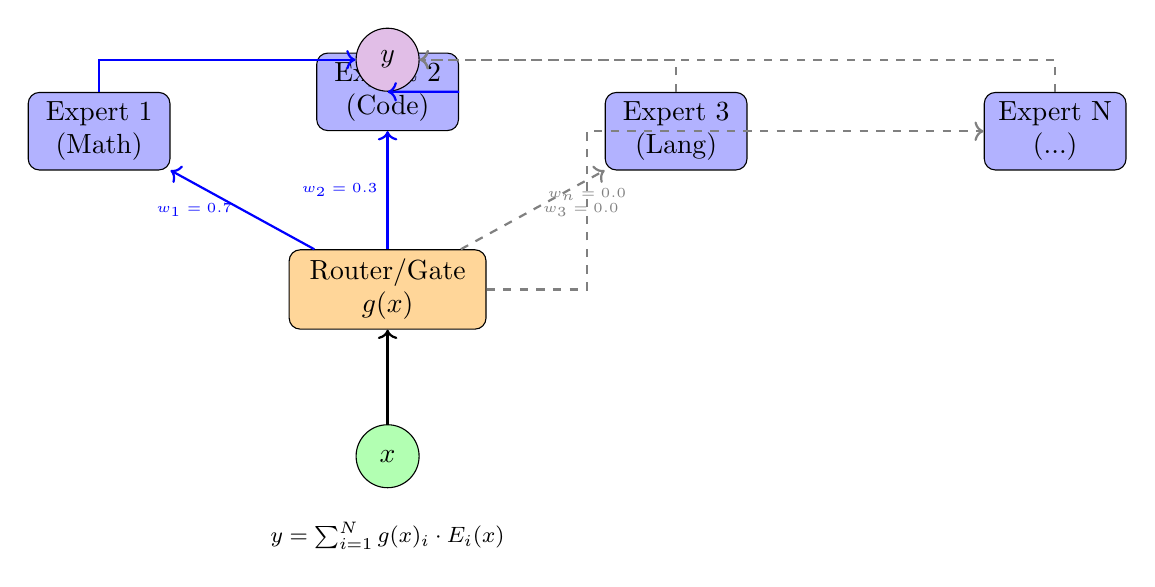
\begin{tikzpicture}[scale=0.85,
    node distance=1.2cm,
    expert/.style={rectangle, rounded corners, draw, fill=blue!30, minimum width=1.8cm, minimum height=0.8cm, align=center},
    router/.style={rectangle, rounded corners, draw, fill=orange!40, minimum width=2.5cm, minimum height=0.8cm, align=center},
    input/.style={circle, draw, fill=green!30, minimum size=0.8cm},
    output/.style={circle, draw, fill=purple!30, minimum size=0.8cm}
]

% Input
\node[input] (input) {$x$};

% Router
\node[router, above=of input] (router) {Router/Gate\\$g(x)$};

% Experts
\node[expert, above left=1cm and 1.5cm of router] (expert1) {Expert 1\\(Math)};
\node[expert, above=1.5cm of router] (expert2) {Expert 2\\(Code)};
\node[expert, above right=1cm and 1.5cm of router] (expert3) {Expert 3\\(Lang)};
\node[expert, right=3cm of expert3] (expertn) {Expert N\\(...)};

% Output aggregation
\node[output, above=2cm of router] (output) {$y$};

% Arrows from input to router
\draw[->, thick] (input) -- (router);

% Arrows from router to experts with weights
\draw[->, thick, blue] (router) -- (expert1) node[midway, left, font=\tiny] {$w_1=0.7$};
\draw[->, thick, blue] (router) -- (expert2) node[midway, left, font=\tiny] {$w_2=0.3$};
\draw[->, thick, gray, dashed] (router) -- (expert3) node[midway, right, font=\tiny] {$w_3=0.0$};
\draw[->, thick, gray, dashed] (router.east) -- ++(1.5,0) |- (expertn.west) node[near start, above, font=\tiny] {$w_n=0.0$};

% Arrows from experts to output
\draw[->, thick, blue] (expert1) |- (output);
\draw[->, thick, blue] (expert2) -- (output);
\draw[->, thick, gray, dashed] (expert3) |- (output);
\draw[->, thick, gray, dashed] (expertn) |- (output);

% Formula
\node[below=0.3cm of input, font=\footnotesize] {$y = \sum_{i=1}^{N} g(x)_i \cdot E_i(x)$};

\end{tikzpicture}
\end{center}

\vspace{0.3em}

\textbf{Typical setup:} N=8-64 experts, but only top-2 are active per token
\end{frame}

\begin{frame}{The Router Mechanism 🎯}
\textbf{How does routing work?}

\vspace{0.5em}

\textbf{Step 1: Compute routing scores}
$$h(x) = W_{\text{gate}} \cdot x$$

\vspace{0.3em}

\textbf{Step 2: Apply softmax to get probabilities}
$$g(x) = \text{softmax}(h(x))$$

\vspace{0.3em}

\textbf{Step 3: Select top-k experts (typically k=2)}
$$\text{Top-k}(g(x)) \rightarrow \{i_1, i_2\}$$

\vspace{0.3em}

\textbf{Step 4: Route token only to selected experts}
$$y = \sum_{i \in \text{top-k}} g(x)_i \cdot E_i(x)$$

\vspace{0.5em}

\textbf{Benefits:}
\begin{itemize}\setlength{\itemsep}{0pt}
    \item ✅ Sparse computation: Only 2 out of N experts active
    \item ✅ Scalable: Can add more experts without increasing per-token cost
    \item ✅ Specialization: Experts learn different capabilities
    \item ✅ Better quality/compute ratio
\end{itemize}
\end{frame}

\begin{frame}[fragile]{MoE in PyTorch (Simplified) 💻}
\begin{lstlisting}[language=Python]
import torch
import torch.nn as nn
import torch.nn.functional as F

class MoELayer(nn.Module):
    def __init__(self, d_model, num_experts, expert_capacity, k=2):
        super().__init__()
        self.num_experts = num_experts
        self.k = k  # Top-k routing

        # Router
        self.gate = nn.Linear(d_model, num_experts)

        # Experts (simple FFN for each)
        self.experts = nn.ModuleList([
            nn.Sequential(
                nn.Linear(d_model, 4 * d_model),
                nn.ReLU(),
                nn.Linear(4 * d_model, d_model)
            )
            for _ in range(num_experts)
        ])

    def forward(self, x):
        # x: (batch_size, seq_len, d_model)
        batch_size, seq_len, d_model = x.shape

        # Compute routing scores
        router_logits = self.gate(x)  # (batch, seq, num_experts)
        router_probs = F.softmax(router_logits, dim=-1)

        # Select top-k experts
        top_k_probs, top_k_indices = torch.topk(router_probs, self.k, dim=-1)
        # top_k_probs: (batch, seq, k)
        # top_k_indices: (batch, seq, k)
\end{lstlisting}
\end{frame}

\begin{frame}[fragile]{MoE Forward Pass (cont.) 💻}
\begin{lstlisting}[language=Python]
        # Initialize output
        output = torch.zeros_like(x)

        # Route to experts
        for i in range(self.k):
            # Get expert indices for this position
            expert_idx = top_k_indices[:, :, i]  # (batch, seq)
            expert_weight = top_k_probs[:, :, i]  # (batch, seq)

            # Process through each expert
            for expert_id in range(self.num_experts):
                # Mask for tokens routed to this expert
                mask = (expert_idx == expert_id)

                if mask.any():
                    # Get tokens for this expert
                    expert_input = x[mask]

                    # Process through expert
                    expert_output = self.experts[expert_id](expert_input)

                    # Add weighted output
                    output[mask] += expert_weight[mask].unsqueeze(-1) * expert_output

        return output
\end{lstlisting}

\vspace{0.3em}
\small
\textit{Note: This is simplified. Production implementations handle batching and load balancing more efficiently.}
\end{frame}

% ============================================================
% SECTION 3: MoE CHALLENGES
% ============================================================
\section{MoE Challenges \& Solutions}

\begin{frame}{Load Balancing Problem ⚖️}
\textbf{Problem:} Some experts get overused, others underutilized

\vspace{0.5em}

\begin{center}
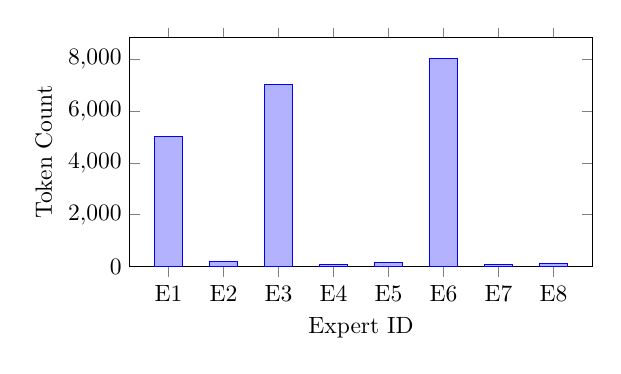
\begin{tikzpicture}[scale=0.85]
    \begin{axis}[
        ybar,
        width=0.7\textwidth,
        height=5cm,
        ylabel={Token Count},
        xlabel={Expert ID},
        symbolic x coords={E1, E2, E3, E4, E5, E6, E7, E8},
        xtick=data,
        ylabel near ticks,
        ymin=0,
        bar width=12pt,
    ]
    \addplot coordinates {
        (E1, 5000)
        (E2, 200)
        (E3, 7000)
        (E4, 100)
        (E5, 150)
        (E6, 8000)
        (E7, 80)
        (E8, 120)
    };
    \end{axis}
\end{tikzpicture}
\end{center}

\vspace{0.3em}

\textbf{Why this is bad:}
\begin{itemize}\setlength{\itemsep}{0pt}
    \item Inefficient use of capacity
    \item Some experts undertrained
    \item Bottlenecks at popular experts
    \item Reduced model expressiveness
\end{itemize}
\end{frame}

\begin{frame}[shrink=10]{Load Balancing Solutions 🔧}
\textbf{1. Auxiliary Load Balancing Loss}

$$\mathcal{L}_{\text{balance}} = \alpha \cdot \sum_{i=1}^{N} f_i \cdot P_i$$

where:
\begin{itemize}\setlength{\itemsep}{0pt}
    \item $f_i$ = fraction of tokens routed to expert $i$
    \item $P_i$ = expert $i$'s average routing probability
    \item $\alpha$ = balancing coefficient (e.g., 0.01)
\end{itemize}

\vspace{0.5em}

\textbf{2. Expert Capacity}
\begin{itemize}\setlength{\itemsep}{0pt}
    \item Limit number of tokens per expert
    \item Capacity $C = \frac{\text{tokens per batch}}{\text{num experts}} \times \text{capacity factor}$
    \item Overflow tokens routed to next-best expert or skipped
\end{itemize}

\vspace{0.5em}

\textbf{3. Random Routing (with probability)}
\begin{itemize}\setlength{\itemsep}{0pt}
    \item Add noise to routing decisions
    \item Prevents complete collapse to few experts
\end{itemize}
\end{frame}

\begin{frame}[shrink=10]{Training Instability ⚠️}
\textbf{Challenges in training MoE:}

\vspace{0.5em}

\begin{enumerate}\setlength{\itemsep}{0pt}
    \item \textbf{Routing Collapse}
    \begin{itemize}\setlength{\itemsep}{0pt}
        \item All tokens routed to one or few experts
        \item \textit{Solution:} Load balancing loss, initialization
    \end{itemize}

    \item \textbf{Expert Imbalance}
    \begin{itemize}\setlength{\itemsep}{0pt}
        \item Some experts undertrained
        \item \textit{Solution:} Balanced batching, capacity limits
    \end{itemize}

    \item \textbf{High Variance Gradients}
    \begin{itemize}\setlength{\itemsep}{0pt}
        \item Discrete routing decisions
        \item \textit{Solution:} Softmax gating, larger batch sizes
    \end{itemize}

    \item \textbf{Dead Experts}
    \begin{itemize}\setlength{\itemsep}{0pt}
        \item Expert never gets activated
        \item \textit{Solution:} Expert dropout, random routing
    \end{itemize}
\end{enumerate}

\vspace{0.5em}

\textbf{Best Practice:} Start with dense model, then convert to MoE for fine-tuning
\end{frame}

\begin{frame}[shrink=10]{Memory and Communication 💾}
\textbf{MoE Memory Requirements:}

\vspace{0.5em}

\begin{alertblock}{Challenge}
All experts must be in memory, even if only 2 are active!
\end{alertblock}

\vspace{0.5em}

\textbf{Example: Mixtral 8x7B}
\begin{itemize}\setlength{\itemsep}{0pt}
    \item 8 experts × 7B parameters each = 56B total
    \item But only 2 experts active → 14B active parameters
    \item \textbf{Memory:} Need to store all 56B parameters
    \item \textbf{Compute:} Only process 14B parameters per token
\end{itemize}

\vspace{0.5em}

\textbf{Solutions:}
\begin{enumerate}\setlength{\itemsep}{0pt}
    \item \textbf{Expert Parallelism}: Distribute experts across GPUs
    \item \textbf{Offloading}: Keep inactive experts on CPU/disk
    \item \textbf{Quantization}: Reduce precision (int8, int4)
    \item \textbf{Shared Experts}: Some experts always active for all tokens
\end{enumerate}
\end{frame}

% ============================================================
% SECTION 4: MIXTRAL CASE STUDY
% ============================================================
\section{Mixtral: MoE in Action}

\begin{frame}[shrink=10]{Mixtral 8x7B 🎬}
\begin{block}{Mixtral (Jiang et al., 2024)}
A state-of-the-art sparse MoE model from Mistral AI with 8 experts, each 7B parameters.
\end{block}

\vspace{0.5em}

\textbf{Architecture:}
\begin{itemize}\setlength{\itemsep}{0pt}
    \item \textbf{Total parameters}: 47B (8 experts × 7B, minus shared layers)
    \item \textbf{Active parameters}: 13B (only 2 experts active per token)
    \item \textbf{Layers}: 32 transformer blocks
    \item \textbf{Context}: 32K tokens
    \item \textbf{Vocabulary}: 32K tokens (SentencePiece)
\end{itemize}

\vspace{0.5em}

\textbf{Training:}
\begin{itemize}\setlength{\itemsep}{0pt}
    \item Open weights (Apache 2.0 license)
    \item Multilingual (English, French, German, Spanish, Italian)
    \item Code-capable
\end{itemize}

\vspace{0.3em}
\small
\textit{Reference: Jiang et al. (2024) - "Mixtral of Experts"}
\end{frame}

\begin{frame}{Mixtral Performance 📊}
\textbf{Comparison with dense models:}

\vspace{0.5em}

\begin{table}
\small
\begin{tabular}{l c c c c}
\toprule
\textbf{Model} & \textbf{Params} & \textbf{Active} & \textbf{MMLU} & \textbf{Speed} \\
\midrule
Llama 2 7B & 7B & 7B & 46.8 & 1.0× \\
Llama 2 13B & 13B & 13B & 55.0 & 0.5× \\
Llama 2 70B & 70B & 70B & 69.7 & 0.16× \\
\textbf{Mixtral 8x7B} & \textbf{47B} & \textbf{13B} & \textbf{70.6} & \textbf{6×} \\
\bottomrule
\end{tabular}
\end{table}

\vspace{0.5em}

\textbf{Key Results:}
\begin{itemize}\setlength{\itemsep}{0pt}
    \item ✅ Matches/exceeds Llama 2 70B quality
    \item ✅ 6× faster inference (13B active vs 70B)
    \item ✅ Better cost/performance ratio
    \item ✅ Fits on fewer GPUs
\end{itemize}

\vspace{0.5em}

\begin{thinkbox}
MoE achieves 70B-model quality with 13B-model inference cost!
\end{thinkbox}
\end{frame}

\begin{frame}[shrink=10]{What Do Experts Learn? 🔬}
\textbf{Do experts actually specialize?}

\vspace{0.5em}

\textbf{Analysis of Mixtral experts:}

\begin{itemize}\setlength{\itemsep}{0pt}
    \item \textbf{Language-specific}: Some experts prefer French vs English
    \item \textbf{Domain-specific}: Code, math, natural language
    \item \textbf{Syntactic}: Different parts of speech
    \item \textbf{Positional}: Some activated more at start/end of sequences
\end{itemize}

\vspace{0.5em}

\textbf{Interesting findings:}
\begin{itemize}\setlength{\itemsep}{0pt}
    \item Specialization emerges without explicit supervision!
    \item Different tokens in same sentence may route to different experts
    \item Some experts are "generalists," others highly specialized
    \item Multilingual data leads to language-specific experts
\end{itemize}

\vspace{0.5em}

\begin{discussionbox}
How could we encourage specific types of specialization during training?
\end{discussionbox}
\end{frame}

% ============================================================
% SECTION 5: OTHER EFFICIENCY TECHNIQUES
% ============================================================
\section{Other Efficiency Techniques}

\begin{frame}[shrink=10]{Model Compression Methods 🗜️}
\textbf{Beyond MoE: Other ways to make models efficient}

\vspace{0.5em}

\begin{enumerate}\setlength{\itemsep}{0pt}
    \item \textbf{Quantization}
    \begin{itemize}\setlength{\itemsep}{0pt}
        \item Reduce precision: FP16, INT8, INT4
        \item 4-bit quantization: 4× memory reduction!
        \item QLoRA: Efficient fine-tuning with quantization
    \end{itemize}

    \item \textbf{Pruning}
    \begin{itemize}\setlength{\itemsep}{0pt}
        \item Remove unimportant weights
        \item Structured (entire layers) vs unstructured (individual weights)
        \item Up to 50-90\% sparsity with minimal quality loss
    \end{itemize}

    \item \textbf{Distillation}
    \begin{itemize}\setlength{\itemsep}{0pt}
        \item Train small model to mimic large model
        \item DistilBERT, DistilGPT
        \item 40\% size, 95\% performance
    \end{itemize}

    \item \textbf{Parameter Sharing}
    \begin{itemize}\setlength{\itemsep}{0pt}
        \item ALBERT: Share weights across layers
        \item Reduces parameters, not computation
    \end{itemize}
\end{enumerate}
\end{frame}

\begin{frame}[shrink=10]{Inference Optimizations ⚡}
\textbf{Making generation faster:}

\vspace{0.5em}

\begin{enumerate}\setlength{\itemsep}{0pt}
    \item \textbf{KV Cache}
    \begin{itemize}\setlength{\itemsep}{0pt}
        \item Store key-value pairs from previous tokens
        \item Avoid recomputing attention for past tokens
        \item Essential for autoregressive generation
    \end{itemize}

    \item \textbf{Flash Attention}
    \begin{itemize}\setlength{\itemsep}{0pt}
        \item Fused attention kernel
        \item 2-4× faster, less memory
        \item FlashAttention-2 even better
    \end{itemize}

    \item \textbf{Speculative Decoding}
    \begin{itemize}\setlength{\itemsep}{0pt}
        \item Use small model to draft tokens
        \item Large model verifies in parallel
        \item 2-3× speedup with no quality loss
    \end{itemize}

    \item \textbf{Batch Processing}
    \begin{itemize}\setlength{\itemsep}{0pt}
        \item Continuous batching (vLLM)
        \item Better GPU utilization
        \item Higher throughput
    \end{itemize}
\end{enumerate}
\end{frame}

\begin{frame}[shrink=10]{State Space Models: Mamba 🐍}
\textbf{Alternative to Transformers with linear-time complexity}

\vspace{0.5em}

\begin{block}{Mamba (Gu \& Dao, 2023)}
State space models that can match Transformer performance with $O(n)$ instead of $O(n^2)$ complexity.
\end{block}

\vspace{0.5em}

\textbf{Why this matters:}
\begin{itemize}\setlength{\itemsep}{0pt}
    \item Attention scales quadratically with sequence length
    \item SSMs scale linearly
    \item Better for long sequences (100K+ tokens)
    \item Faster training and inference
\end{itemize}

\vspace{0.5em}

\textbf{Trade-offs:}
\begin{itemize}\setlength{\itemsep}{0pt}
    \item ❌ Less expressive than full attention (for some tasks)
    \item ❌ Newer, less mature
    \item ✅ Much more efficient
    \item ✅ Can combine with attention in hybrid models
\end{itemize}

\vspace{0.3em}
\small
\textit{Reference: Gu \& Dao (2023) - "Mamba: Linear-Time Sequence Modeling with Selective State Spaces"}
\end{frame}

\begin{frame}[shrink=5]{Efficiency Trade-off Landscape 🗺️}
\begin{center}
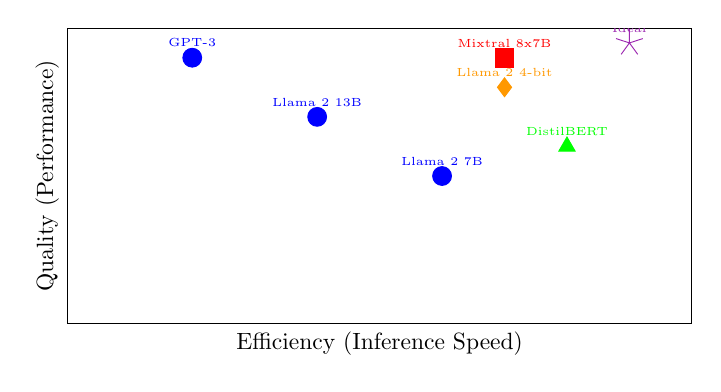
\begin{tikzpicture}[scale=0.85]
    \begin{axis}[
        width=0.9\textwidth,
        height=6cm,
        xlabel={Efficiency (Inference Speed)},
        ylabel={Quality (Performance)},
        xmin=0, xmax=10,
        ymin=0, ymax=10,
        xtick=\empty,
        ytick=\empty,
        grid=major,
    ]

    % Dense models
    \addplot[only marks, mark=*, mark size=4pt, blue] coordinates {
        (2, 9)  % Large dense
        (4, 7)  % Medium dense
        (6, 5)  % Small dense
    };
    \node[blue] at (axis cs:2,9.5) {\tiny GPT-3};
    \node[blue] at (axis cs:4,7.5) {\tiny Llama 2 13B};
    \node[blue] at (axis cs:6,5.5) {\tiny Llama 2 7B};

    % MoE models
    \addplot[only marks, mark=square*, mark size=4pt, red] coordinates {
        (7, 9)  % MoE
    };
    \node[red] at (axis cs:7,9.5) {\tiny Mixtral 8x7B};

    % Distilled models
    \addplot[only marks, mark=triangle*, mark size=4pt, green] coordinates {
        (8, 6)  % Distilled
    };
    \node[green] at (axis cs:8,6.5) {\tiny DistilBERT};

    % Quantized
    \addplot[only marks, mark=diamond*, mark size=4pt, orange] coordinates {
        (7, 8)  % Quantized
    };
    \node[orange] at (axis cs:7,8.5) {\tiny Llama 2 4-bit};

    % Ideal point
    \addplot[only marks, mark=star, mark size=6pt, purple] coordinates {
        (9, 9.5)
    };
    \node[purple] at (axis cs:9,10) {\tiny Ideal};

    \end{axis}
\end{tikzpicture}
\end{center}

\vspace{0.3em}

\textbf{Key Insight:} Different techniques for different use cases!
\end{frame}

% ============================================================
% SECTION 6: SUSTAINABILITY
% ============================================================
\section{Sustainability \& Accessibility}

\begin{frame}{Environmental Impact 🌍}
\textbf{The carbon cost of large language models:}

\vspace{0.5em}

\begin{table}
\small
\begin{tabular}{l c c}
\toprule
\textbf{Model} & \textbf{Training CO$_2$ (tons)} & \textbf{Equivalent} \\
\midrule
BERT & 652 & 1 passenger: SF $\leftrightarrow$ NY (125×) \\
GPT-3 & 502 & 112 cars for 1 year \\
Llama 2 & ~539 & 120 cars for 1 year \\
\bottomrule
\end{tabular}
\end{table}

\vspace{0.5em}

\textbf{Factors affecting carbon footprint:}
\begin{itemize}\setlength{\itemsep}{0pt}
    \item Model size (more parameters = more compute)
    \item Training time
    \item Hardware efficiency (newer GPUs more efficient)
    \item Energy source (coal vs solar)
    \item Location of data center
\end{itemize}

\vspace{0.5em}

\small
\textit{Source: Strubell et al. (2019) - "Energy and Policy Considerations for Deep Learning in NLP"}
\end{frame}

\begin{frame}[shrink=10]{Democratizing Access 🔓}
\begin{discussionbox}
Should powerful AI be accessible to everyone, or only large organizations?
\end{discussionbox}

\vspace{0.5em}

\textbf{Current reality:}
\begin{itemize}\setlength{\itemsep}{0pt}
    \item Training GPT-3 scale model: \$4-12M
    \item Requires 1000+ GPUs
    \item Only big tech companies can afford
    \item Creates AI "haves" and "have-nots"
\end{itemize}

\vspace{0.5em}

\textbf{Efficiency enables democratization:}
\begin{itemize}\setlength{\itemsep}{0pt}
    \item ✅ Smaller models on consumer hardware
    \item ✅ Open-source weights (Llama, Mixtral, Mistral)
    \item ✅ Efficient fine-tuning (LoRA, QLoRA)
    \item ✅ Cloud access with pay-per-use pricing
    \item ✅ Edge deployment (on-device models)
\end{itemize}

\vspace{0.5em}

\begin{alertblock}{Goal}
Make AI accessible to researchers, startups, and developing nations—not just big tech!
\end{alertblock}
\end{frame}

\begin{frame}[shrink=10]{Open vs Closed Models 🤔}
\begin{columns}[T]
\begin{column}{0.48\textwidth}
\textbf{Closed (GPT-4, Claude):}
\begin{itemize}\setlength{\itemsep}{0pt}
    \item ✅ Better safety control
    \item ✅ Monetization easier
    \item ✅ Protect IP
    \item ✅ Can update/improve
    \item ❌ No transparency
    \item ❌ Vendor lock-in
    \item ❌ Limited customization
    \item ❌ Privacy concerns
\end{itemize}
\end{column}

\begin{column}{0.48\textwidth}
\textbf{Open (Llama, Mixtral):}
\begin{itemize}\setlength{\itemsep}{0pt}
    \item ✅ Transparency
    \item ✅ Community innovation
    \item ✅ Full control
    \item ✅ No API costs
    \item ✅ Privacy (on-prem)
    \item ❌ Potential misuse
    \item ❌ Compute requirements
    \item ❌ Need ML expertise
\end{itemize}
\end{column}
\end{columns}

\vspace{0.5em}

\textbf{The debate:}
\begin{itemize}\setlength{\itemsep}{0pt}
    \item Mirrors open-source software vs proprietary
    \item But higher stakes (safety, dual-use concerns)
    \item Trend: Moving toward more open models
    \item Efficiency helps open models (smaller = easier to distribute)
\end{itemize}
\end{frame}

% ============================================================
% SECTION 7: FUTURE DIRECTIONS
% ============================================================
\section{Future Directions}

\begin{frame}[shrink=10]{Future of Efficient LLMs 🔮}
\textbf{Where is the field heading?}

\vspace{0.5em}

\begin{enumerate}\setlength{\itemsep}{0pt}
    \item \textbf{Hybrid Architectures}
    \begin{itemize}\setlength{\itemsep}{0pt}
        \item Combine MoE + attention + SSMs
        \item Use different mechanisms for different parts
        \item Dynamic architecture selection
    \end{itemize}

    \item \textbf{Conditional Computation}
    \begin{itemize}\setlength{\itemsep}{0pt}
        \item Adjust depth/width based on input difficulty
        \item Early exit for easy examples
        \item More compute for hard problems
    \end{itemize}

    \item \textbf{Neural Architecture Search}
    \begin{itemize}\setlength{\itemsep}{0pt}
        \item Automatically find efficient architectures
        \item Multi-objective optimization (quality + speed + size)
    \end{itemize}

    \item \textbf{Hardware Co-Design}
    \begin{itemize}\setlength{\itemsep}{0pt}
        \item Design models for specific hardware
        \item Custom chips for LLMs (TPUs, Groq, Cerebras)
        \item Edge-specific models
    \end{itemize}
\end{enumerate}
\end{frame}

\begin{frame}[shrink=10]{Key Takeaways 🔑}
\begin{enumerate}\setlength{\itemsep}{0pt}
    \item \textbf{MoE enables efficient scaling}
    \begin{itemize}\setlength{\itemsep}{0pt}
        \item More parameters, fewer active per token
        \item Better quality/compute ratio
    \end{itemize}

    \vspace{0.2em}

    \item \textbf{Challenges exist but solvable}
    \begin{itemize}\setlength{\itemsep}{0pt}
        \item Load balancing, training instability
        \item Solutions: auxiliary losses, capacity limits
    \end{itemize}

    \vspace{0.2em}

    \item \textbf{Mixtral proves MoE works at scale}
    \begin{itemize}\setlength{\itemsep}{0pt}
        \item 70B-quality with 13B-cost
        \item Open weights accelerate adoption
    \end{itemize}

    \vspace{0.2em}

    \item \textbf{Many paths to efficiency}
    \begin{itemize}\setlength{\itemsep}{0pt}
        \item Quantization, pruning, distillation
        \item Flash attention, speculative decoding
        \item SSMs, hybrid architectures
    \end{itemize}

    \vspace{0.2em}

    \item \textbf{Efficiency enables democratization}
    \begin{itemize}\setlength{\itemsep}{0pt}
        \item Lower costs, environmental impact
        \item Accessible to more researchers
    \end{itemize}
\end{enumerate}
\end{frame}

\begin{frame}[shrink=10]{Readings 📖}
\textbf{Required:}
\begin{enumerate}\setlength{\itemsep}{0pt}
    \item \textbf{Shazeer et al. (2017)}: Outrageously Large Neural Networks: The Sparsely-Gated Mixture-of-Experts Layer
    \href{https://arxiv.org/abs/1701.06538}{[arXiv]}

    \item \textbf{Jiang et al. (2024)}: Mixtral of Experts
    \href{https://arxiv.org/abs/2401.04088}{[arXiv]}
\end{enumerate}

\vspace{0.5em}

\textbf{Recommended:}
\begin{itemize}\setlength{\itemsep}{0pt}
    \item Fedus et al. (2022): Switch Transformers \href{https://arxiv.org/abs/2101.03961}{[arXiv]}
    \item Gu \& Dao (2023): Mamba \href{https://arxiv.org/abs/2312.00752}{[arXiv]}
    \item Dao et al. (2022): FlashAttention \href{https://arxiv.org/abs/2205.14135}{[arXiv]}
    \item Strubell et al. (2019): Energy and Policy Considerations \href{https://arxiv.org/abs/1906.02243}{[arXiv]}
    \item HuggingFace MoE Blog \href{https://huggingface.co/blog/moe}{[Blog]}
\end{itemize}
\end{frame}

\begin{frame}
\begin{center}
\Huge{Questions? 💬}

\vspace{2cm}

\Large{Next: Ethics, Bias, and Safety!}
\end{center}
\end{frame}

\end{document}
